\section{Vektorgeometrie}
		  Generell gilt auf dieser Zusammenfassung: \\
			
			\begin{tabular}{ll}
			$\vec{p}$ & Ortsvektor (Vektor vom Ursprung zu Punkt auf Geraden)\\
			$\vec{r}$ & Richtungsvektor \\
			$\vec{x}$ & Platzhalter für Punkt (auf Ebene / Geraden) $x_1, x_2, x_3$ \\
			$s, t, u, v$ & Variablen $\in \mathbb{R}$ \\
			\end{tabular}						
			
			
			\subsection{Normalenvektor}		    
		   	Der Normalenvektor einer Geraden / Ebene steht senkrecht auf der Geraden / Ebene.	\\
		   	Der Normalenvektor kann mit dem Vektorprodukt oder dem  \\
		   	Skalarprodukt berechnet werden\\
		   	\\
		   	\begin{tabular}{ll}
		   	Vektorprodukt: & $\vec{n} =  \vec{r_1} \times \vec{r_2}$ \\
		   	Skalarpodukt: & $\vec{n} \bullet \vec{r_1} = 0$ und $\vec{n} \bullet \vec{r_2} = 0$  \\
		   	& Skalarprodukte als Gleichung aufschreiben \\
		   	& $\rightarrow$ Gauss-Tableau  $\rightarrow$ Normalenvektor \\
		   	& (es gibt eine frei wählbare Variable) \\
			\end{tabular}		   			
			
			
		    \subsection{Darstellungsformen von Ebenen / Geraden}	
		    
			\subsubsection{Koordinatenform}	% unsicher ob korrekt
			\begin{tabular}{lll}
			Ebene: & $\textcolor{red}{n_x} \, x_1 + \textcolor{red}{n_y} \, x_2 + \textcolor{red}{n_z} \, x_3 = b$ & $\textcolor{red}{5} \, x_1 + \textcolor{red}{10} \, x_2 \textcolor{red}{- 2} \, x_3 = 6 $ \\
			\\
			Gerade: &  $\textcolor{red}{n_x} \, x_1 + \textcolor{red}{n_y} \, x_2  = b$ & $\textcolor{red}{5} \, x_1 + \textcolor{red}{10} \, x_2 = 6 $ \\
			\\
			\end{tabular}						    

		    Die roten Koeffizienten entsprechen den Koordinaten des \\
		    Normalenvektors. \\
		    $b$ entspricht dem Abstand der Ebene zum Nullpunkt des \\
		    Koordinatensystems.
	    
	    
	
		    
		    
			\subsubsection{Parameterform}
			Hinweis: in 2 Dimensionen ohne z-Koordinate, ansonsten analog \\			
			
			Gerade g: \quad $\vec{p} + s \cdot \vec{r} = \begin{pmatrix} p_x \\ p_y \\ p_z \end{pmatrix}	+ t \cdot \begin{pmatrix} r_x \\ r_y \\ r_z \end{pmatrix}$ \\
			\\

			Ebene E: \quad $\vec{p} + s \cdot \vec{r_1} + t \cdot \vec{r_2} = \begin{pmatrix} p_x \\ p_y \\ p_z \end{pmatrix}	+ s \cdot \begin{pmatrix} r1_x \\ r1_y \\ r1_z \end{pmatrix} + t \cdot \begin{pmatrix} r2_x \\ r2_y \\ r3_z \end{pmatrix}$ 
			
			
			\subsubsection{Normalenform}		   
			\begin{minipage}{0.48\linewidth}
			Gerade g: \quad $\vec{n} \bullet (\vec{x} - \vec{p}) = 0$ \\
			\end{minipage}	
			\hfill	
			\begin{minipage}{0.48\linewidth}
			Ebene E: \quad $\vec{n} \bullet (\vec{x} - \vec{p}) = 0$ \\
			\end{minipage}	 
		    
			Wenn $\neq 0$ liegt der Punkt x nicht auf der Geraden / Ebene 
			
			
		    \subsubsection{Umrechnungen der verschiedenen Formen}
		    \textbf{Koordinatenform in Parameterform}\\
		    \\
		    \begin{tabular}{ll}
		    1. & Normalenvektor aus Koordinatengleichung ablesen \\
		    & Koordinatengleichung einsetzen \\
		    2. & Richtungsvektoren aus den 3 Punkten bilden \\
		    3. & Parameterform aufstellen \\
		    \\
		    \end{tabular}
		    

		    	\textbf{Koordinatenform in Normalenform} \\
		    	\\
		    	\begin{tabular}{ll}
		    1. & 3 Punkte auf Ebene bestimmen  Spurpunkte in \\
		    & Koordinatengleichung einsetzen \\
		    2. & Punkt auf Ebene finden: Spurpunkt einsetzen \\
		    3. & Aus gefundenem Normalen- und Richtungsvektor \\
		    & Normalenform aufstellen \\
		    \\
		    \end{tabular}
		    
		    
			\textbf{Parameterform in Normalenform}\\
		    	\\
		    	\begin{tabular}{ll}
		    1. & aus Richtungsvektoren den Normalenvektor bilden \\
		    2. & Aus gefundenem Normalenvektor und bekanntem Stützvektor \\
		    &  die Normalenform aufstellen \\	   
		    \\
		    \end{tabular}		    
		    
		    
		    	\textbf{Parameterform in Koordinatenform}\\
			\\
		    	\begin{tabular}{ll}
		    1. &  Paramaterform Zeile für Zeile als einzelne Gleichungen \\
		    & aufschreiben \\
		    2. &  Variablen s und t schrittweise aus GlSys eliminieren  \\
		    & Vielfache einer Gleichung mit Vielfache von anderer Gleichung \\
		    & addieren/subtrahieren und somit neue Gleichungen finden \\
		    3. &  Wenn s und t eliminiert sind und die Schlussgleichung \\
		    & gefunden ist, entspricht dies der Koordinatengleichung  \\
		    \\
		    \end{tabular}		    	 
		    
		    	\textbf{Normalenform in Parameterform} \\
		    	\\
		    	\begin{tabular}{ll}
		    1. & Richtungsvektoren aus Normalenvektor finden:\\
		    & Eine Komponente des Normalenvektors 0 setzen \\
		    & $\rightarrow$ 0 in erstem Richtungsvektor \\
		    & verbleibenden Komponenten vertauscht in Richtungsvektor \\
		    & einsetzen und ein Vorzeichen tauschen \\
		    2. & Schritt 1 für zweiten Richtungsvektor wiederholen  \\
		    & Wichtig: Andere Komponente von Normalen 0 setzen! \\
		    3. & Aus Richtungsvektoren und bekannten Stützvektor \\
		    &  Parameterform aufstellen  \\	   
		    \end{tabular}	    
		    		    
		    	\vfill\null
		    	\columnbreak	    
		    		    
		    		    
		    		    
		    \subsection{Hesse'sche Normalform als Darstellungsform}
		    \textbf{In der Hesse'schen Normalform ist der Abstand d vom \\
		    Nullpunkt zur Ebene immer d = 1} 
		    
		    \subsubsection{Beispiel Umwandlung in Hessesche Normalform}
		    \begin{tabular}{ll}
		    Ebene E: & $3 x_1 + 8 x_2 - 5 x_3 = 3$ \\
		    \\
		    Hesse'sche Normalform: & $x_1 + \frac{8}{3} x_2 - \frac{5}{3} x_3 = 1$
		    \end{tabular}
		    
			
			\subsection{Orthonormalbasis}
			In einer Orthonormalbasis stehen die Basisvektoren $b_i$ senkrecht \\
			aufeinander und haben die Länge 1 \\
			\\
			Ausgedrückt mit dem Skalarprodukt bedeutet dies: \\
			\begin{tabular}{ll}
			Senkrecht aufeinander: & $\vec{b_1} \bullet \vec{b_2} = 0$ \\
			Länge 1: & $\vec{b_1} \bullet \vec{b_1} = 1$
			\end{tabular}
		  
		   
			\subsection{Skalarprodukt}
			
			\begin{minipage}{0.4\linewidth}
			\textbf{2 Dimensionen} \\
			\\
			$\vec{a} \bullet \vec{b} = \vert \vec{a} \vert \cdot \vert \vec{b} \vert \cdot \cos(\alpha)$ \\
			\\
			\\
			\\
			\\
			\end{minipage}
			\hfill
			\begin{minipage}{0.58\linewidth}
			\textbf{3 Dimensionen} \\
			\\
			$\vec{a} \bullet \vec{b} = \begin{pmatrix} a_x \\ a_y \\ a_z \end{pmatrix} \bullet \begin{pmatrix} b_x \\ b_y \\ b_z \end{pmatrix}$ \\
			\\
			wenn Basis = Orthonormalbasis!\\
			\end{minipage}
			
			

			\subsubsection{Eigenschaften des Skalarprodukts}
			
			\begin{tabular}{ll}
			Linearität & linear in $\vec{a}$ und $\vec{b}$ (bilinear) \\
			& $\rightarrow$ man kann ausmultiplizieren\\
			
			Orthagonalität: &  $\vec{a} \bullet \vec{b} = 0$ \\
			
			Länge im Quadrat: & $\vec{a} \bullet \vec{b} = \vert \vec{u} \vert ^2$ 	\\
						
			Länge: &$\sqrt{\vec{a} \bullet \vec{a}}$ \\
			
			Als Matrixprodukt: & $\vec{a}^t \vec{b} = \vec{b}^t \vec{a} = \vec{a} \bullet \vec{b}$ \\
			\\
			\end{tabular}
			
			\textbf{Winkel zwischen zwei Vektoren} \\
			\\
			$\cos(\alpha) = \frac{\vec{a} \bullet \vec{b}}{ \vert \vec{a} \vert \cdot \vert \vec{b} \vert}$ \\
			
			
			 
		    \subsection{Länge (Betrag) eines Vektors}
		    $\vert \vec{a} \vert = \sqrt{\vec{a} \bullet \vec{a}} = \sqrt{a_x^2 + a_y^2 + a_z^2}$
		    
		    \vfill\null
		    \columnbreak
		    
		    
			
			\subsection{Orthagonale Projektion mittels Skalarprodukt}
			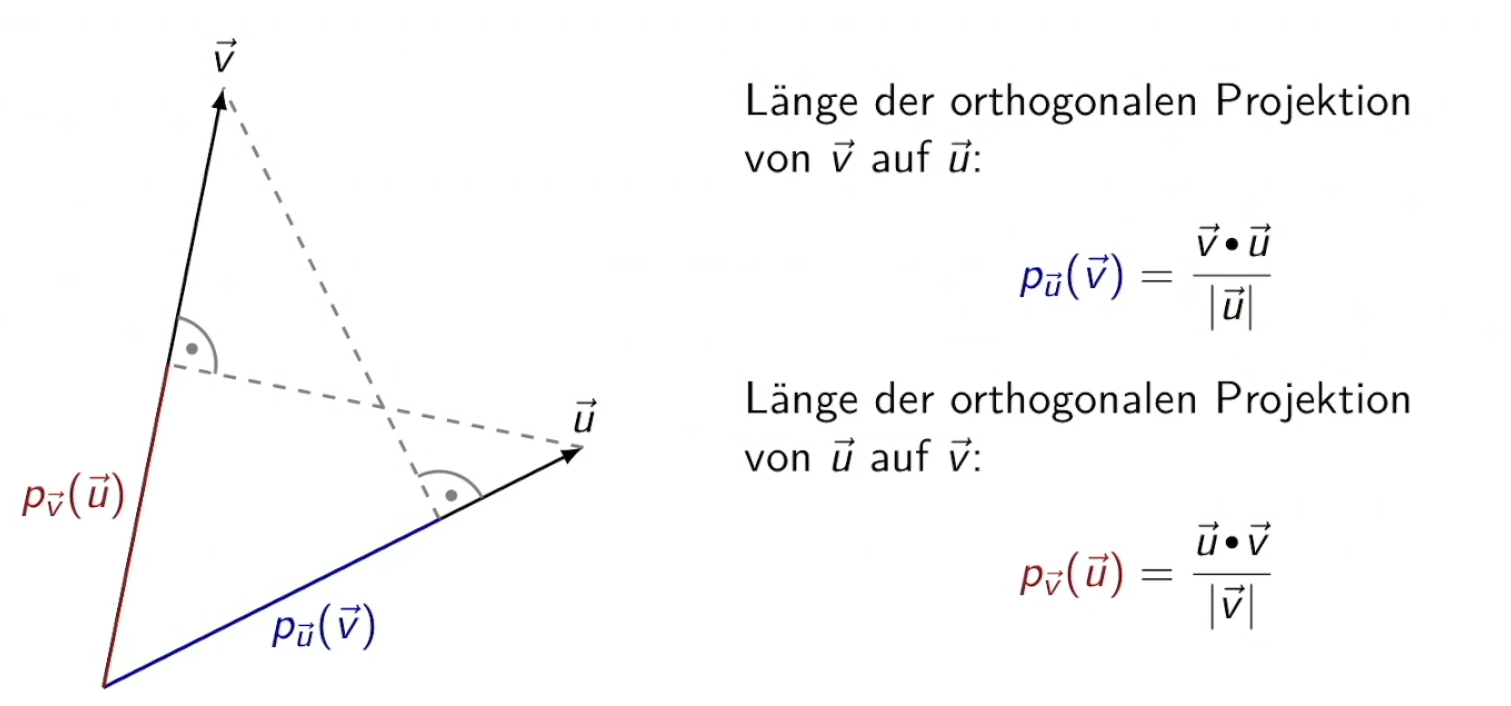
\includegraphics[width=0.65\linewidth]{Bilder/orthagonale-projektion}
			
			
			\subsection{Prallel- und Orthagonalkomponente}
			Ein Vektor kann in zwei orthagonale Komponenten aufgeteilt werden \\					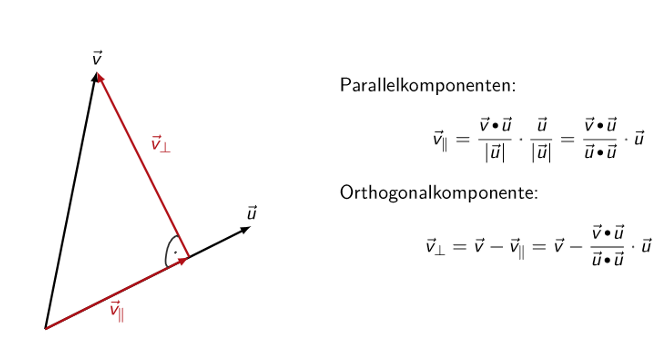
\includegraphics[width=0.65\linewidth]{Bilder/parallel-orthagonal}
			
			
			\subsection{Spiegelung}
			Der gespiegelte Vektor entspricht $\vec{v'} = \vec{v} - 2 \vec{v_{\parallel}} = \vec{v} - 2 \vec{n} \frac{\vec{n} \bullet \vec{v}}{\vert \vec{n} \vert ^2} $ \\
			\begin{minipage}[b]{.5\linewidth} 
  			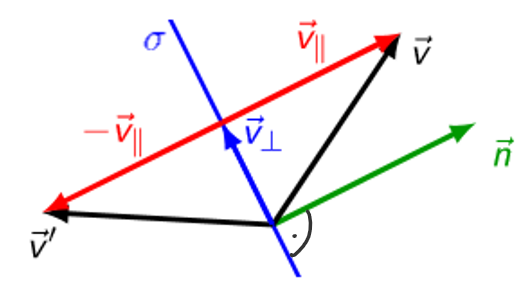
\includegraphics[width=\linewidth]{Bilder/spiegelung}
			\end{minipage}
			\hfill
			\begin{minipage}[b]{.45\linewidth} 
			Beschreibung der \\
			Spiegelnugsmatrix S: \\
			\\
			$S = E - 2 \frac{1}{\vert \vec{n} \vert ^2} \vec{n} \bullet \vec{n}^t$  	\\
			\\
			Wenn $\vec{n}$  Länge 1 hat: \\
			$S = E - 2 \vec{n}^0 \bullet \vec{n}^{0 t}$  	
			\end{minipage}						
			
			\subsection{Orthagonale Matrix / Orthagonalität}
			\textbf{Orthagonal heisst: $A^t A = E$}\\		
			Eine orthagonale Matrix ändert das Skalarprodukt nicht. \\
			\\
			Eigenschaften orthagonale Matritzten: \\
			\begin{tabular}{lll}
			$A^t A = E$ & $A^{-1} = A^t$ & $A^t$ auch orthagonal
			\end{tabular}
				
			
			\subsection{Hessesche Normalform}
			\textbf{Berechnung Abstand d von Punkt $\vec{x}$ zu Ebene}  \\
			Anwendung in Koordinatenform und Normalform möglich \\
			$\vec{q}$ entspricht dem Stützvektor der Ebene! 
			
			\subsubsection{Länge des Normalenvektors nicht 1}
			
			\begin{tabular}{lll}
			\textbf{Koordinatenform} & & \textbf{Parameterform} \\
			\\
			
			$d = \frac{n_x}{\vert \vec{n} \vert} x_1 + \frac{n_y}{\vert \vec{n} \vert} x_2 + \frac{n_z}{\vert \vec{n} \vert} x_3 - \frac{\vec{n} \bullet \vec{q}}{\vert \vec{n} \vert}$ & & $d = \frac{\vec{n} \bullet (\vec{x} - \vec{q})}{\vert \vec{n} \vert}$ \\
			\end{tabular}
			
			\vfill\null
			\columnbreak
			
			
			\subsubsection{Länge des Normalenvektors ist 1}
			
			\begin{tabular}{lll}
			\textbf{Koordinatenform} & & \textbf{Parameterform} \\
			\\
			
			$d = n_x x_1 + n_y x_2 + n_z x_3 - \vec{n} \bullet \vec{q}$ & & $d = \vec{n} \bullet (\vec{x} - \vec{q}) $
			\end{tabular}
				    
		    
		    
		    
			\subsection{Vektorprodukt (Kreuzprodukt)}		    
		    \textbf{Nur definiert in 3 Dimensionen!} \\
		    \\
		    \begin{minipage}{0.45\linewidth}
		    $\vec{a} \times \vec{b} = \begin{pmatrix} a_2 b_3 - a_3 b_2 \\ -(a_1 b_3 - a_3 b_1) \\ a_1 b_2 - a_2 b_2 \end{pmatrix}$ \\
		    \end{minipage}
		    \hfill
		    \begin{minipage}{0.5\linewidth}
		    $\vec{a} \times \vec{b} = -\vec{b} \times \vec{a}$ \\
		    $\vec{a} \times \vec{a} = 0$ \\
		    $\vec{a} \times (\vec{b} \times \vec{c}) = (\vec{a} \bullet \vec{c}) \vec{b} - (\vec{a} \bullet \vec{b}) \vec{b}$ \\
		    $(\vec{a} \times \vec{b}) \times \vec{c} = (\vec{a} \bullet \vec{c}) \vec{b} - (\vec{a} \bullet \vec{b}) \vec{b}$
		    \end{minipage}
		    
		    
		    \subsubsection{Eigenschaften des Vektorprodukts}
		    
		    \begin{tabular}{ll}
		    $\bullet$ & $\vec{a} \times \vec{b}$ ist senkrecht auf $\vec{a}$ und $\vec{b}$\\
		    & $( \vec{a} \times \vec{b}) \bullet \vec{a} = \det(\vec{a}, \vec{b}, \vec{a}) = 0$\\
		    & $( \vec{a} \times \vec{b}) \bullet \vec{b} = \det(\vec{a}, \vec{b}, \vec{b}) = 0$\\
		    $\bullet$ & $\vert \vec{a} \times \vec{b} \vert$ ist Fläche eines Parallelogramm \\ 
		    $\bullet$ & $\vec{a}, \, \vec{b}, \, \vec{a} \times \vec{b}$ bilden ein Rechtssystem \\
		    $\bullet$ & $\vert \vec{a} \times \vec{b} \vert ^2 = (\vec{b} \times \vec{a}) \cdot (\vec{a} \times \vec{b}) = \det(\vec{a}, \, \vec{b}, \, \vec{a} \times \vec{b})$  ist Volumen\\
		    &  eines Parallelepipeds \\
		    $\bullet$ & Höhe eines Parallelogramms: $\frac{\vert \vec{a} \times \vec{b} \vert}{\vec{a}}$ \\
		      $\bullet$ & Zwischenwinkel eines Parallelogramms: $\sin(\alpha) = \frac{h}{\vert \vec{b} \vert} = \frac{\vert \vec{a} \times \vec{b} \vert}{\vert \vec{a} \vert \bullet \vert \vec{b} \vert}$ \\
		    \end{tabular}
		    
		    \includegraphics[width= 0.3\linewidth]{Bilder/Zwischenwinkel}

		    
		    \subsection{Berechnung von Polygonen (Schuhbändelformel)}
		    Die Fläche eines Polygons kann aus Flächen von Dreiecken, als über Determinanten berechnet werden: \\
		    \\
		    \begin{minipage}{0.48\linewidth}
		    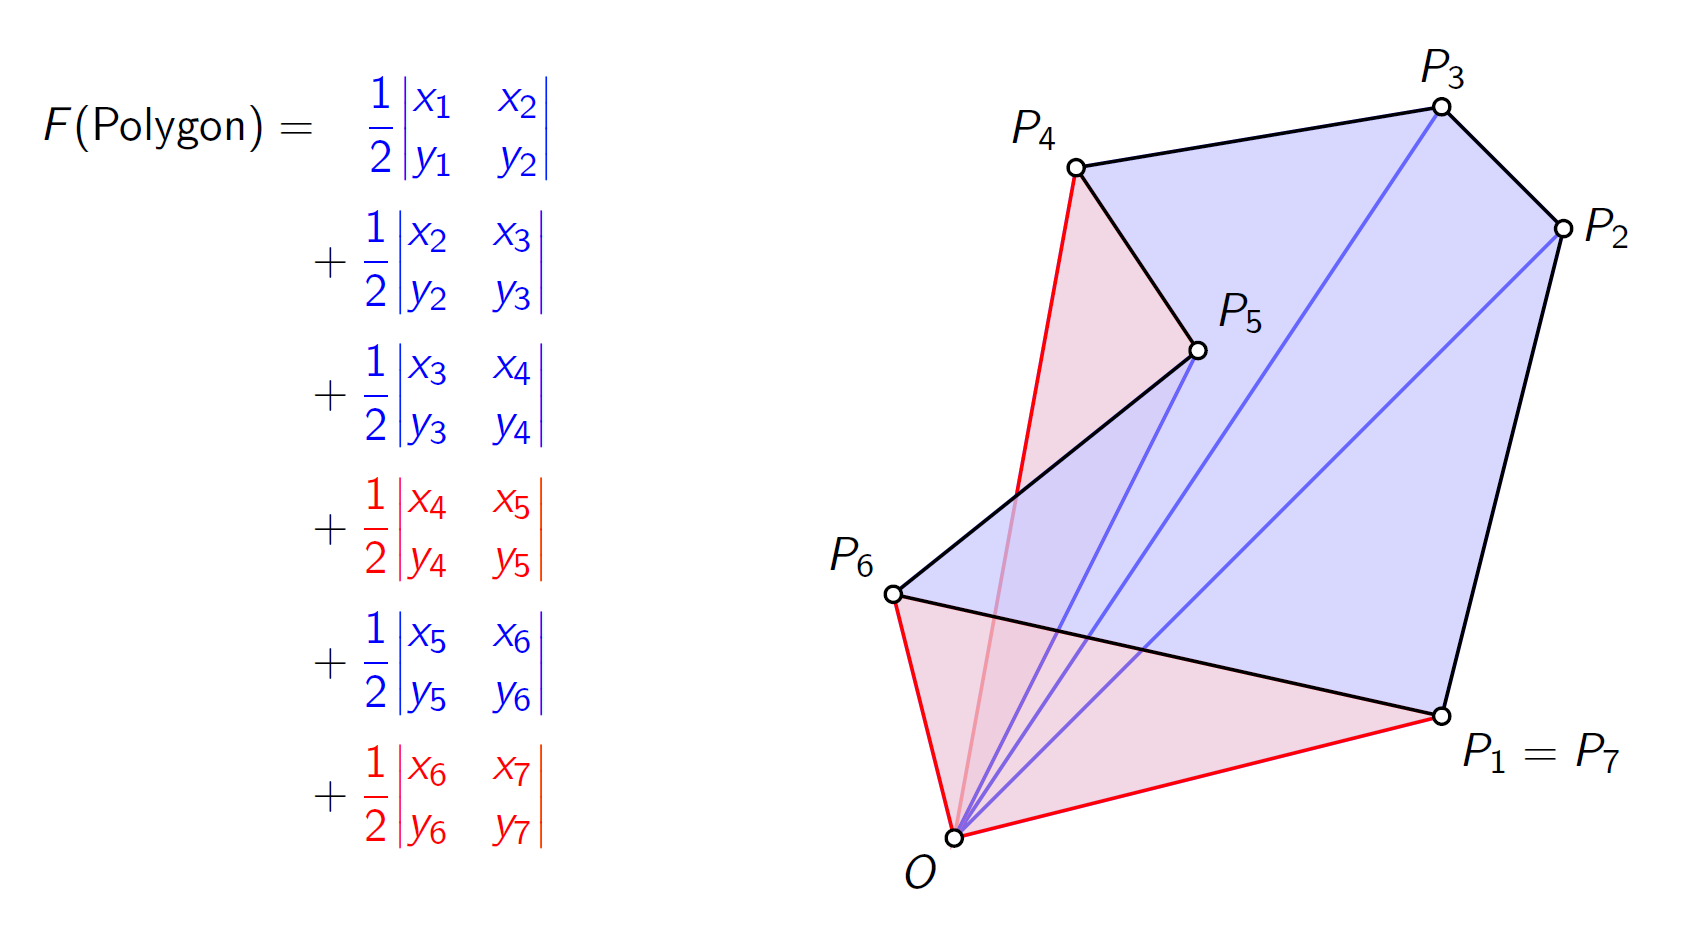
\includegraphics[width=\linewidth]{Bilder/flaeche-polygon} \\
		    \end{minipage}
		    \hfill
		    \begin{minipage}{0.48\linewidth}
		    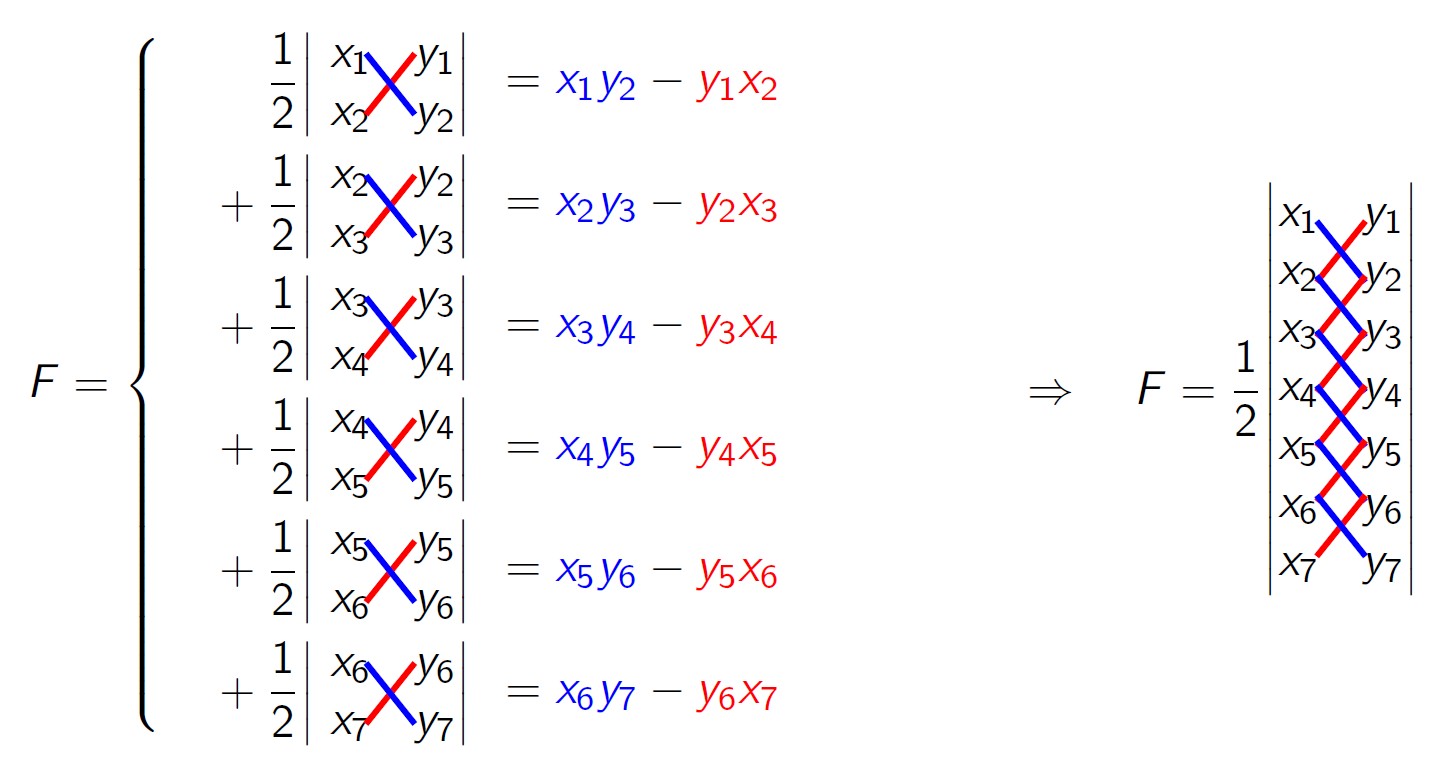
\includegraphics[width=\linewidth]{Bilder/schuhbaendel}
		    \end{minipage}

		    
		    \vfill\null
		    \columnbreak


		    

		    
			\subsection{Allgemeine Lösung für Schnittprobleme}	
			Um ein Schnittproblem zu lösen kann alles in ein Gauss-Tableau \\
			geschrieben werden, welches anschliessend gelöst werden kann. \\
			\\
			\begin{tabular}{ll}
			$E$ & Einheitsmatrix  \\ 
			$\vec{u}, \vec{v}$ & Richtungsvektoren \\
			$\vec{p_1}, \vec{p_1} $ & Stützvektoren \\
			\end{tabular}
			
			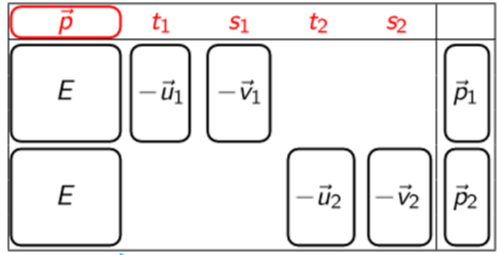
\includegraphics[width=0.7\linewidth]{Bilder/schnittpunkt-tableau} 
			
			
			\subsubsection{Beispiel: Schnittpunkt von zwei Geraden}
			
			
		$\textcolor{blue}{\begin{pmatrix} x_1 \\ x_2 \\ x_3 \end{pmatrix} = \begin{pmatrix} 18 \\ -7 \\ 0 \end{pmatrix} + s \cdot \begin{pmatrix} 7 \\ -2 \\ 1\end{pmatrix}}$ \qquad $\textcolor{orange}{\begin{pmatrix} x_1 \\ x_2 \\ x_3 \end{pmatrix} = \begin{pmatrix} -18 \\ 19 \\ 7 \end{pmatrix} + t \cdot \begin{pmatrix} -3 \\ 4 \\ 2\end{pmatrix}}$ \\
		
		\vspace{0.2cm}
		
		\begin{minipage}[b]{.5\linewidth} 
  		\begin{tabular}{| c c c c c | c |}
		\hline
		$x_1$ & $x_2$ & $x_3$ & $s$ & $t$ & \\
		\hline
		\textcolor{blue}1 & \textcolor{blue}0 & \textcolor{blue}0 & \textcolor{blue}{-7} & \textcolor{blue}0 & \textcolor{blue}{18} \\
		\textcolor{blue}0 & \textcolor{blue}1 & \textcolor{blue}0 & \textcolor{blue}2 & \textcolor{blue}0 & \textcolor{blue}{-7} \\
		\textcolor{blue}0 & \textcolor{blue}0 & \textcolor{blue}1 & \textcolor{blue}{-1} & \textcolor{blue}0 & \textcolor{blue}0 \\
		\textcolor{orange}1 & \textcolor{orange}0 & \textcolor{orange}0 & \textcolor{orange}0 & \textcolor{orange}3 & \textcolor{orange}{-18} \\
		\textcolor{orange}0 & \textcolor{orange}1 & \textcolor{orange}0 & \textcolor{orange}0 & \textcolor{orange}{-4} & \textcolor{orange}{19} \\
		\textcolor{orange}0 & \textcolor{orange}0 & \textcolor{orange}1 & \textcolor{orange}0 & \textcolor{orange}{-2} & \textcolor{orange}7 \\
	    \hline
		\end{tabular}		
  		\end{minipage}
		\hfill
		\begin{minipage}[b]{.45\linewidth} 
  		\begin{tabular}{| c c c c c | c |}
		\hline
		$x_1$ & $x_2$ & $x_3$ & $s$ & $t$ & \\
		\hline
		1 & 0 & 0 & 0 & 0 & -3 \\
		0 & 1 & 0 & 0 & 0 & -1 \\
		0 & 0 & 1 & 0 & 0 & -3 \\
		0 & 0 & 0 & 1 & 0 & -3 \\
		0 & 0 & 0 & 0 & 1 & -5 \\
		0 & 0 & 0 & 0 & 0 & 0 \\
	    \hline
		\end{tabular}		
		\end{minipage}		
		
		\vspace{0.2cm}
		
		Schnittpunkt: ($-3$ $\vert$ $-1$ $\vert$ $-3$) \quad $s = -3$ \quad $t = -5$	
		
		
		
		
		\subsubsection{Beispiel: Durchstosspunkt Gerade durch Ebene}
		    
		 $\textcolor{blue}{\begin{pmatrix} x_1 \\ x_2 \\ x_3 \end{pmatrix} = \begin{pmatrix} 0 \\ 0 \\ 1 \end{pmatrix} + s \cdot \begin{pmatrix} 1 \\ 1 \\ -1\end{pmatrix}}$ \quad $\textcolor{orange}{\begin{pmatrix} x_1 \\ x_2 \\ x_3 \end{pmatrix} = \begin{pmatrix} 0 \\ 0 \\ 0 \end{pmatrix} + u \cdot \begin{pmatrix} 1 \\ 0 \\ 1\end{pmatrix} + v \cdot \begin{pmatrix} 0 \\ 1 \\ 1\end{pmatrix}}$ \\
		\\

  		\begin{tabular}{| c c c c c c | c |}
		\hline
		$x_1$ & $x_2$ & $x_3$ & $s$ & $u$ & $v$ & \\
		\hline
		\textcolor{blue}1 & \textcolor{blue}0 & \textcolor{blue}0 & \textcolor{blue}{-1} & \textcolor{blue}0 & \textcolor{blue}0 &  \textcolor{blue}0 \\
		\textcolor{blue}0 & \textcolor{blue}1 & \textcolor{blue}0 & \textcolor{blue}{-1} & \textcolor{blue}0 & \textcolor{blue}0 &  \textcolor{blue}0 \\
		\textcolor{blue}0 & \textcolor{blue}0 & \textcolor{blue}1 & \textcolor{blue}1 & \textcolor{blue}0 & \textcolor{blue}0 &  \textcolor{blue}1 \\
		\textcolor{orange}1 & \textcolor{orange}0 & \textcolor{orange}0 & \textcolor{orange}0 & \textcolor{orange}{-1} & \textcolor{orange}0 & \textcolor{orange}0 \\
		\textcolor{orange}0 & \textcolor{orange}1 & \textcolor{orange}0 & \textcolor{orange}0 & \textcolor{orange}0 & \textcolor{orange}{-1} & \textcolor{orange}0 \\
		\textcolor{orange}0 & \textcolor{orange}0 & \textcolor{orange}1 & \textcolor{orange}0 & \textcolor{orange}{-1} & \textcolor{orange}{-1} & \textcolor{orange}0 \\
	    \hline
		\end{tabular}		


  		\begin{tabular}{| c c c c c c | c |}
		\hline
		$x_1$ & $x_2$ & $x_3$ & $s$ & $u$ & $v$ & \\
		\hline
		1 & 0 & 0 & 0 & 0 & 0 & $\frac{1}{3}$ \\
		0 & 1 & 0 & 0 & 0 & 0 & $\frac{1}{3}$ \\
		0 & 0 & 1 & 0 & 0 & 0 & $\frac{2}{3}$ \\
		0 & 0 & 0 & 1 & 0 & 0 & $\frac{1}{3}$ \\
		0 & 0 & 0 & 0 & 1 & 0 & $\frac{1}{3}$ \\
		0 & 0 & 0 & 0 & 0 & 1 & $\frac{1}{3}$\\
	    \hline
		\end{tabular}		
	
	\vspace{0.2cm}
	
		Durchstosspunkt: ($\frac{1}{3} \vert \frac{1}{3} \vert \frac{2}{3}$) \quad $s = \frac{1}{3}$ \quad $u = \frac{1}{3}$ \quad $v =  \frac{1}{3}$	
						
	
	
	
			\subsubsection{Beispiel: Schnittgerade von 2 Ebenen}		    					$\textcolor{blue}{\begin{pmatrix} x_1 \\ x_2 \\ x_3 \end{pmatrix} = \begin{pmatrix} 6 \\ 4 \\ 7 \end{pmatrix} + s \cdot \begin{pmatrix} 3 \\ -2 \\ 2\end{pmatrix} + t \cdot \begin{pmatrix} -5 \\ 3 \\ -7\end{pmatrix}}$ \\
			
			\vspace{0.2cm}
			
			 $\textcolor{orange}{\begin{pmatrix} x_1 \\ x_2 \\ x_3 \end{pmatrix} = \begin{pmatrix} 2 \\ 2 \\ 4 \end{pmatrix} + u \cdot \begin{pmatrix} 4 \\ 11 \\ 0\end{pmatrix} + v \cdot \begin{pmatrix} -1 \\ 1 \\ 3\end{pmatrix}}$ \\
		\\

  		\begin{tabular}{| c c c c c c c | c |}
		\hline
		$x_1$ & $x_2$ & $x_3$ & $s$ & $t$ & $u$ & $v$ &  \\
		\hline
		\textcolor{blue}1 & \textcolor{blue}0 & \textcolor{blue}0 & \textcolor{blue}{-3} & \textcolor{blue}5 & \textcolor{blue}0 & \textcolor{blue}0 & \textcolor{blue}6\\
		\textcolor{blue}0 & \textcolor{blue}1 & \textcolor{blue}0 & \textcolor{blue}2 & \textcolor{blue}{-3} & \textcolor{blue}{0} & \textcolor{blue}0 & \textcolor{blue}4\\
		\textcolor{blue}0 & \textcolor{blue}0 & \textcolor{blue}1 & \textcolor{blue}{-2} & \textcolor{blue}7 & \textcolor{blue}0 & \textcolor{blue}0 & \textcolor{blue}7 \\
		\textcolor{orange}1 & \textcolor{orange}0 & \textcolor{orange}0 & \textcolor{orange}0 & \textcolor{orange}0 & \textcolor{orange}{-4} & \textcolor{orange}1 & \textcolor{orange}2 \\
		\textcolor{orange}0 & \textcolor{orange}1 & \textcolor{orange}0 & \textcolor{orange}0 & \textcolor{orange}0 & \textcolor{orange}{-11} & \textcolor{orange}{-1} & \textcolor{orange}2 \\
		\textcolor{orange}0 & \textcolor{orange}0 & \textcolor{orange}1 & \textcolor{orange}0 & \textcolor{orange}0 & \textcolor{orange}0 & \textcolor{orange}{-3} & \textcolor{orange}4 \\
		\hline
		\end{tabular}		
 
  		\begin{tabular}{| c c c c c c c | c |}
		\hline
		$x_1$ & $x_2$ & $x_3$ & $s$ & $t$ & $u$ & $v$ & \\
		\hline
		1 & 0 & 0 & 0 & 0 & 0 & 1 & $\frac{10}{3}$\\
		0 & 1 & 0 & 0 & 0 & 0 & -1 & $\frac{17}{3}$\\
		0 & 0 & 1 & 0 & 0 & 0 & -3 & 4\\
		0 & 0 & 0 & 1 & 0 & 0 & 2 & $-\frac{1}{3}$\\
		0 & 0 & 0 & 0 & 1 & 0 & 1 & $\frac{1}{3}$\\
		0 & 0 & 0 & 0 & 0 & 1 & 0 & $\frac{1}{3}$\\
		\hline
		\end{tabular}		
		
		\vspace{0.2cm}

		Schnittgerade: $\begin{pmatrix} x_1 \\ x_2 \\ x_3 \end{pmatrix} = \begin{pmatrix} \frac{10}{3} \\ \frac{17}{3} \\ 4 \end{pmatrix} + v \cdot \begin{pmatrix} -1 \\ 1 \\ 3 \end{pmatrix} $
		
		 
			
			\subsection{Orthonormalisierung}
			Beschreibt, wie man von einer beliebigen Basis zu einer \\			
			Orthonormalbasis kommt \\		
			Orthonormalbasis: siehe Abschnitt 4.4 \\
			
			
			\subsubsection{Gram-Schmidtsches Orthonormalisierungsverfahren}
			Basisvektoren $\vec{a_1}$, $\vec{a_2}$ und $\vec{a_3}$ sind nicht orthagonal. Sie sollen \\
			orthagonalisiert werden und durch die Vektoren $\vec{b_1}$, $\vec{b_2}$ und $\vec{b_3}$ \\
			ausgedrückt werden: \\
			
			\begin{tabular}{ll}
			$\vec{b_1}$ = $\frac{\vec{a_1}}{\vert \vec{a_1} \vert}$ & $\vec{b_2}$  = $\frac{\vec{a_2} - ( \vec{a_2} \bullet \vec{b_1} ) \vec{b_1}}{\vert \vec{a_2} - ( \vec{a_2} \bullet \vec{b_1} ) \vec{b_1} \vert}$\\
		 \\
			$\vec{b_3}$ = $\frac{\vec{a_3} - ( \vec{a_3} \bullet \vec{b_1} ) \vec{b_1} - ( \vec{a_3} \bullet \vec{b_2} ) \vec{b_2}}  {\vec{a_3} - ( \vec{a_3} \bullet \vec{b_1} ) \vec{b_1} - ( \vec{a_3} \bullet \vec{b_2} ) \vec{b_2}}$  &  kann beliebig weitergeführt werden \\
			\\
			\end{tabular}
					
					
			\vfill\null
			\columnbreak			
			
			
			\subsection{Least Squares Überbestimmtes Gleichungssystem}
			Ein Gleichungssystem mit mehr Gleichungen als Unbekannten ist im allgemeinen nicht lösbar \\	
			Wir suchen also eine Lösung, welche am ''wenigsten falsch'' ist bzw. $\vert A \cdot \vec{x} - \vec{b} \vert$ möglichst klein 
				
			\subsubsection{Beispiel Least Squares}
			Die Unbekannten sind \textcolor{red}{rot} eingefärbt \\
			\\
			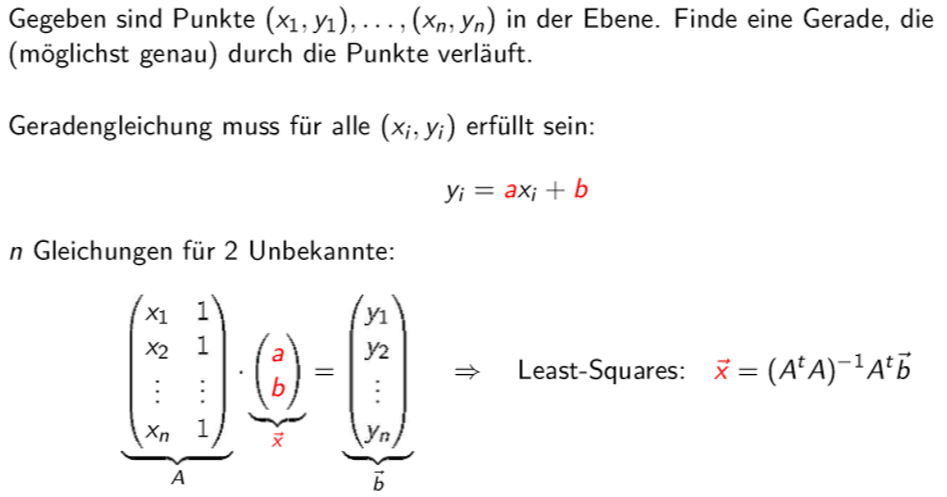
\includegraphics[width=0.8\linewidth]{Bilder/least-squares}\\
			\\
			\textbf{nichtlineare Teile (z.B. $d^2$) können einfach neu benannt weden ($d^2 = m$) und in das Verfahren eingesetzt werden.} \\
			Sobald eine lineare Lösung gefunden ist kann der nichtlineare Teil berechnet werden.
			
			
			\subsection{Kreis und Kugel}		
			
			\subsubsection{Kreis}
			\begin{tabular}{ll}
			Vektorgleichung: & $(\vec{p} - \vec{m})^2 = r^2$\\
			Koordinatengleichung: & $(x- m_x)^2 + (y-m_y)^2 = r^2$\\
			\\
			\end{tabular}
			
			Die Koeffizienten von $x$ und $y$ entsprechen Koordinatenmittelpunkt: \\
			$x^2 - 2 \textcolor{red}{m_x} x + m_x^2 + y^2 - 2 \textcolor{red}{m_y} y + m_y^2 = r^2 $		\\
			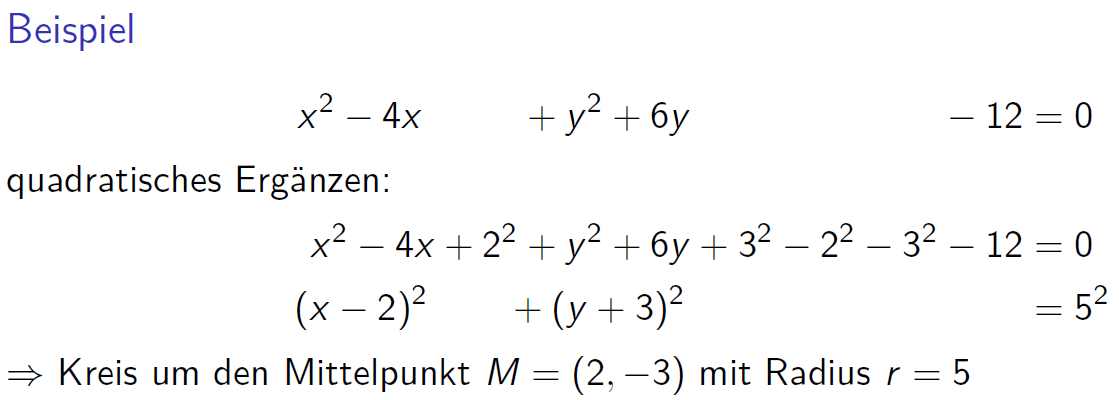
\includegraphics[width=0.8\linewidth]{Bilder/kreisgleichung}	\\
			
			\subsubsection{Thales-Kreis}
			\begin{minipage}[b]{.45\linewidth} 
  			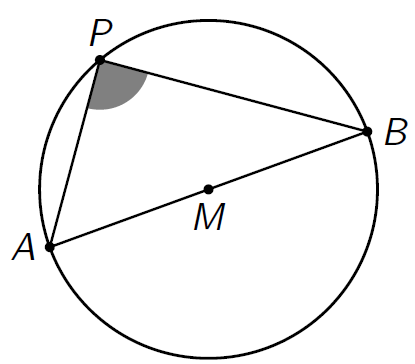
\includegraphics[width=0.7\linewidth]{Bilder/thales-kreis}
			\end{minipage}
			\hfill
			\begin{minipage}[b]{.5\linewidth} 
  			Thales-Kreis: \\
  			\\
  			$\left( \vec{p} - \frac{\vec{a} + \vec{b}}{2} \right) ^2 = \left( \frac{\vec{a} - \vec{b}}{2} \right) ^2 = r^2$	\\
  			\\
  			\\
			\end{minipage}		
			
			\vfill\null
			\columnbreak			
			
			
			\subsubsection{Durchstosspunkt Gerade-Kreis}
				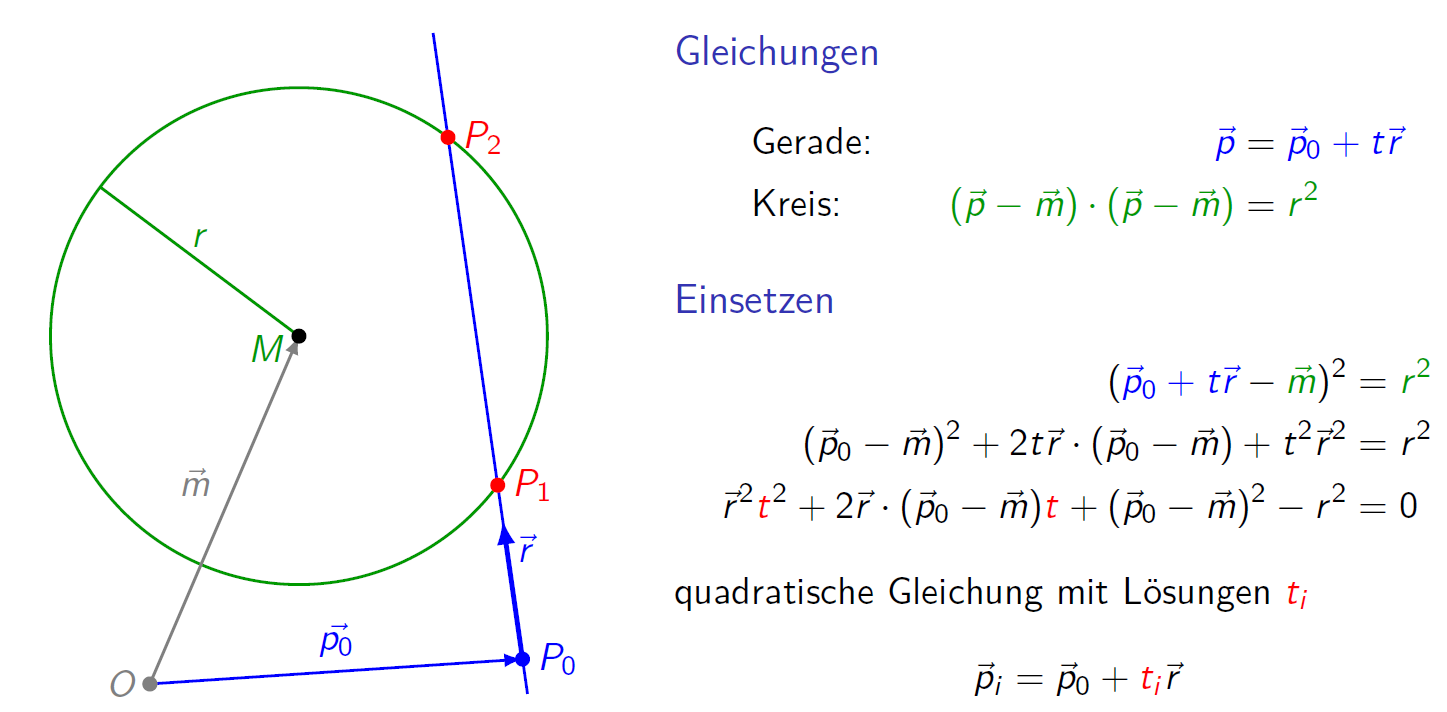
\includegraphics[width=0.8\linewidth]{Bilder/durchstosspunkt-gerade-kreis}	
			
			\subsubsection{Tangente an Kreis}
			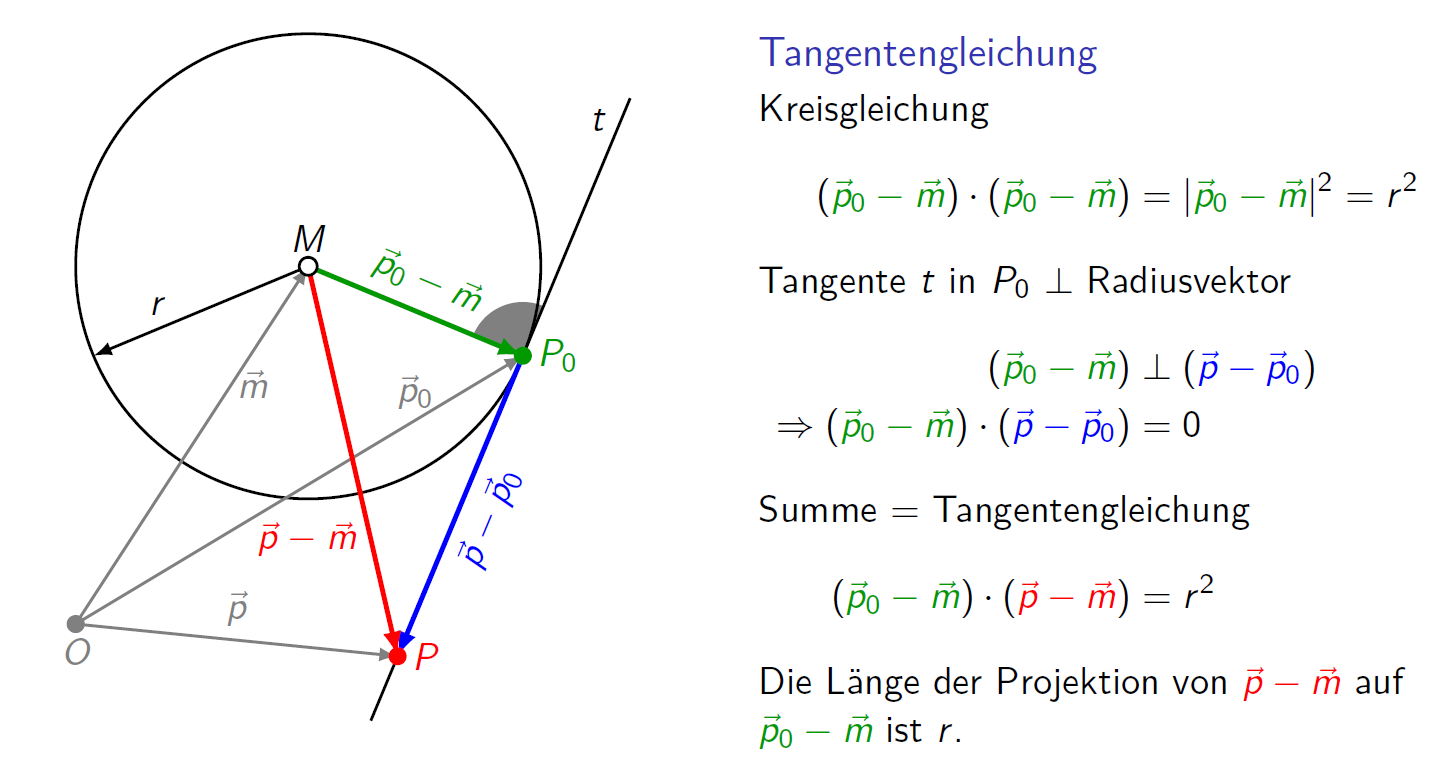
\includegraphics[width=0.8\linewidth]{Bilder/kreis-tangente}	
			
			
			\subsubsection{Kugel}
			\begin{tabular}{ll}
			Vektorgleichung: & $(\vec{p} - \vec{m})^2 = r^2$\\
			Koordinatengleichung: & $(x - m_x)^2 + (y - m_y)^2 + (z - m_z)^2 = r^2$\\
			\end{tabular}
			
			\subsubsection{Zusammenfassung Kugel}
			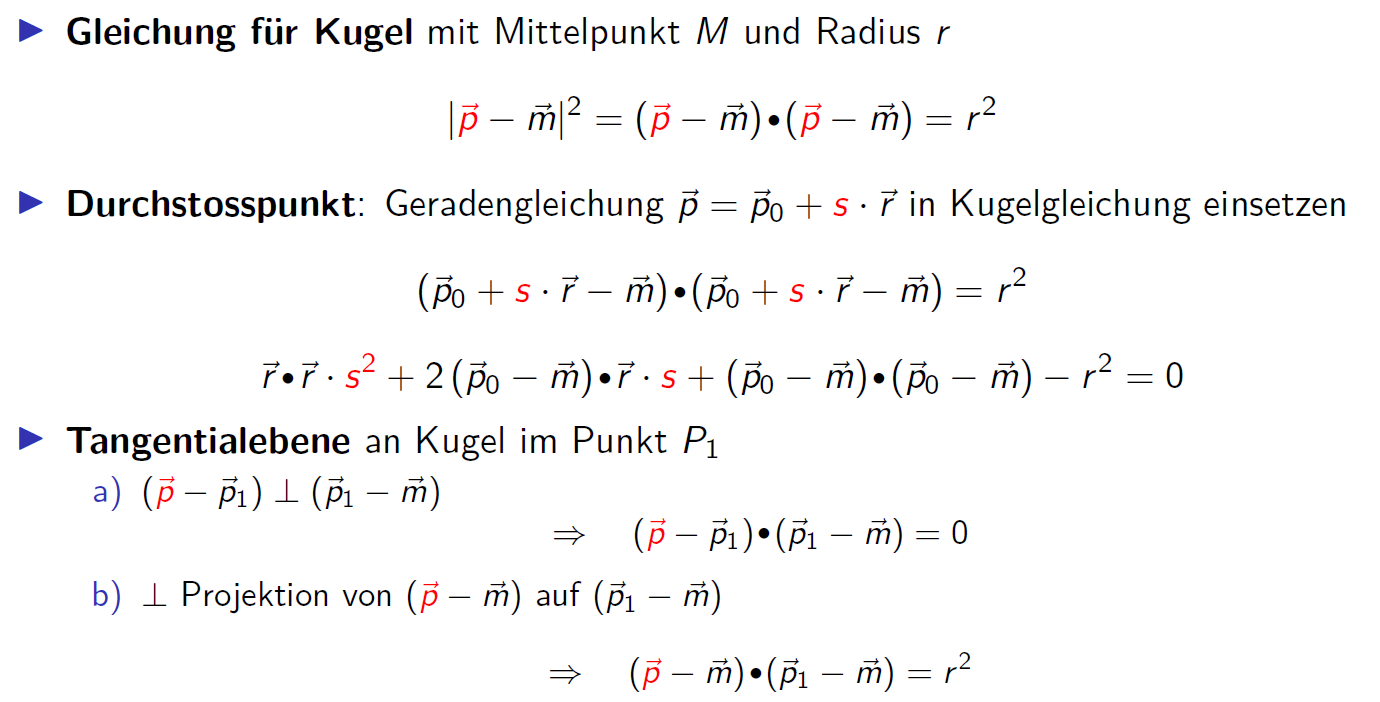
\includegraphics[width=0.8\linewidth]{Bilder/kugel}	
			
			
			\vfill\null
			\columnbreak	
			
			
			
			\subsection{Abstandsprobleme}
		
		\subsubsection{Abstand Punkt-Ebene}
		Berechnung mittels Hessescher Normalform 
		
		
		\subsubsection{Abstand Punkt-Gerade}
		Der Abstand $h$ zwischen der Geraden $g$ und dem Punkt $Q$ entspricht dem Lot zur Geraden $g$ durch $Q$ \\
		Gerade in Paramterdarstellung: $\vec{p} = \vec{p_0} + t \vec{r}$ \\
		 
		 \begin{minipage}{0.45\linewidth}
		 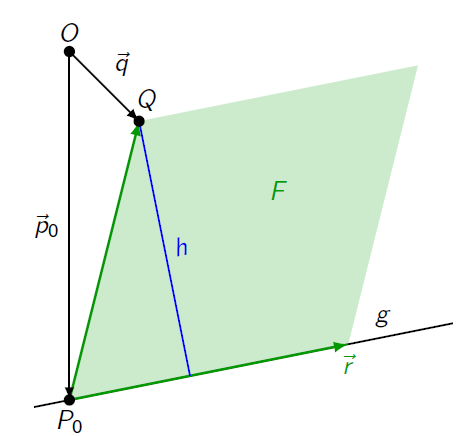
\includegraphics[width=0.6\linewidth]{Bilder/punkt-gerade}
		 \end{minipage}
		\hfill
		\begin{minipage}{0.45\linewidth}
		 $$h = \frac{F}{\vline \vec{r} \vline} =  \frac{r \times ( \vline \vec{q} - \vec{p_0} \vline )}{\vline \vec{r} \vline} $$
		 \end{minipage}

			\subsubsection{Abstand windschiefer Geraden in 3D} 
			Zwei Geraden in Parameterdarstellung:\\					$\vec{p} = \vec{p_0} + t \vec{r_1}$ und $\vec{q} = \vec{q_0} + 2 \vec{r_2}$ \\
			die sich nicht schneiden und nicht parallel sind \\
			
		Abstand $d = (\vec{q_0} -\vec{p_0}) \bullet \frac{\vec{r_1} \times \vec{r_2}}{\vert \vec{r_1} \times \vec{r_2} \vert} $
		
		
		\subsubsection{Minimaler Abstand}
			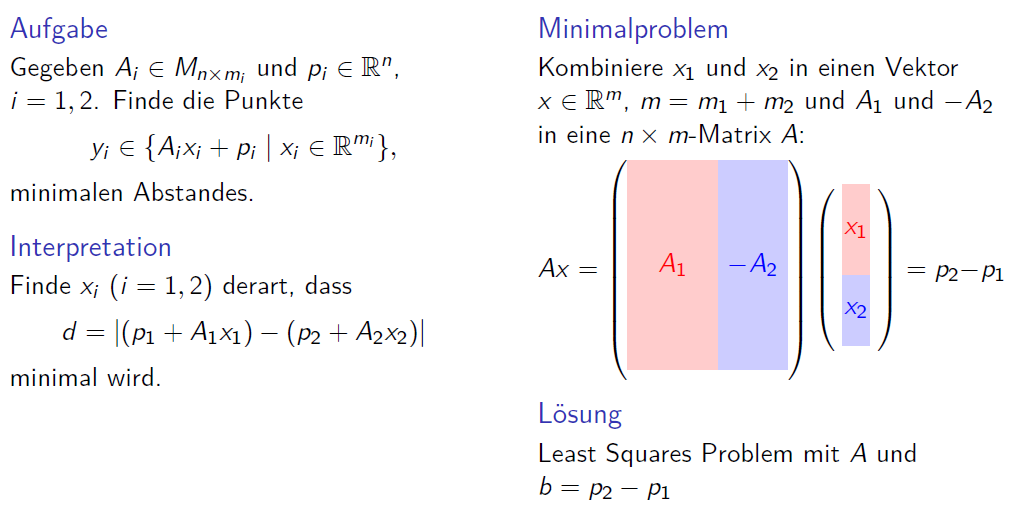
\includegraphics[width=0.9\linewidth]{Bilder/minimaler-abstand}	
		
		
		\vfill\null
		\columnbreak	
		